\documentclass[timestamp,acmtog]{acmart}

\usepackage{booktabs} % For formal tables
%\usepackage{subfigure}
\usepackage{subcaption}
\usepackage{graphicx}
\usepackage{tikz}
\usepackage{wrapfig}
\usepackage{bm}
\newcommand{\ba}{\mathbf{a}}
\newcommand{\bb}{\mathbf{b}}
\newcommand{\bc}{\mathbf{c}}
\newcommand{\bg}{\mathbf{g}}
\newcommand{\br}{\mathbf{r}}
\newcommand{\bff}{\mathbf{f}}
\newcommand{\bv}{\mathbf{v}}
\newcommand{\be}{\mathbf{e}}
\newcommand{\bd}{\mathbf{d}}
\newcommand{\bF}{\mathbf{F}}
\newcommand{\Id}{\mathbf{I}}
\newcommand{\bJ}{\mathbf{J}}
\newcommand{\bx}{\mathbf{x}}
\newcommand{\bw}{\mathbf{w}}
\DeclareMathOperator{\tr}{tr}
\newcommand{\hn}{\hat{\mathbf{n}}}
\newcommand{\fT}{\mathcal{T}}
\newcommand{\bmm}{\mathbf{m}}
\newcommand{\bs}{\mathbf{s}}
\newcommand\todo[1]{\textcolor{red}{#1}}

\acmPrice{15.00}

% The next six lines come directly from the completed rights form.
% You MUST replace them with the lines specific to your accepted work.
\setcopyright{acmlicensed}
\acmJournal{TOG}
\acmYear{2018}\acmVolume{37}\acmNumber{4}\acmArticle{1}\acmMonth{8} \acmDOI{10.1145/3197517.3201395}


% Use the "authoryear" citation style, and make sure citations are in [square brackets].
\citestyle{acmauthoryear}
\setcitestyle{square}

% A useful command for controlling the number of authors per row.
% The default value of "authorsperrow" is 2.
\settopmatter{authorsperrow=2}

% end of preamble.

\begin{document}

% Title. 
% If your title is long, consider \title[short title]{full title} - "short title" will be used for running heads.
\title{Physical Simulation of Environmentally Induced Thin Shell Deformation}

% Authors.
\author{Hsiao-yu Chen}
\affiliation{%
  \institution{University of Texas at Austin}}
  
  \author{Arnav Sastry}
\affiliation{%
  \institution{University of Texas at Austin}}
  
  \author{Wim van Rees}
\affiliation{%
  \institution{Massachusetts Institute of Technology}}  

\author{Etienne Vouga}
\affiliation{%
  \institution{University of Texas at Austin}}

% This command defines the author string for running heads.
%\renewcommand{\shortauthors}{DeJohnette, Rowland-Smith, Badeeri, and Foyt}

% abstract
\begin{abstract}
We present a physically accurate low-order elastic shell model that incorporates active material response to dynamically changing stimuli such as heat, moisture, and growth. Our continuous formulation of the geometrically non-linear elastic energy derives from the principles of differential geometry, and as such naturally incorporates shell thickness, non-zero rest curvature, and physical material properties. By modeling the environmental stimulus as local, dynamic changes in the rest metric of the material, we are able to solve for the corresponding shape changes by integrating the equations of motions given this non-Euclidean rest state. We present models for differential growth and shrinking due to moisture and temperature gradients along and across the surface, and incorporate anisotropic growth by defining an intrinsic machine direction within the material. Comparisons with experiments and volumetric finite elements show that our simulations achieve excellent qualitative and quantitative agreement. By combining the reduced-order shell theory with appropriate physical models, our approach accurately captures all the physical phenomena while avoiding expensive volumetric discretization of the shell volume. 
\end{abstract}

%CCS
\begin{CCSXML}
%<ccs2012>
%<concept>
%<concept_id>10010147.10010371.10010372</concept_id>
%<concept_desc>Computing methodologies~Rendering</concept_desc>
%<concept_significance>500</concept_significance>
%</concept>
%<concept>
%<concept_id>10010147.10010371.10010372.10010374</concept_id>
%<concept_desc>Computing methodologies~Ray tracing</concept_desc>
%<concept_significance>500</concept_significance>
%</concept>
%</ccs2012>
\end{CCSXML}

%\ccsdesc[500]{Computing methodologies~Rendering}
%\ccsdesc[500]{Computing methodologies~Ray tracing}
%
%%keywords
%\keywords{ray tracing, global illumination, octrees, quadtrees}
%
% A "teaser" figure, centered below the title and authors and above the body of the work.
\begin{teaserfigure}
  \centering
  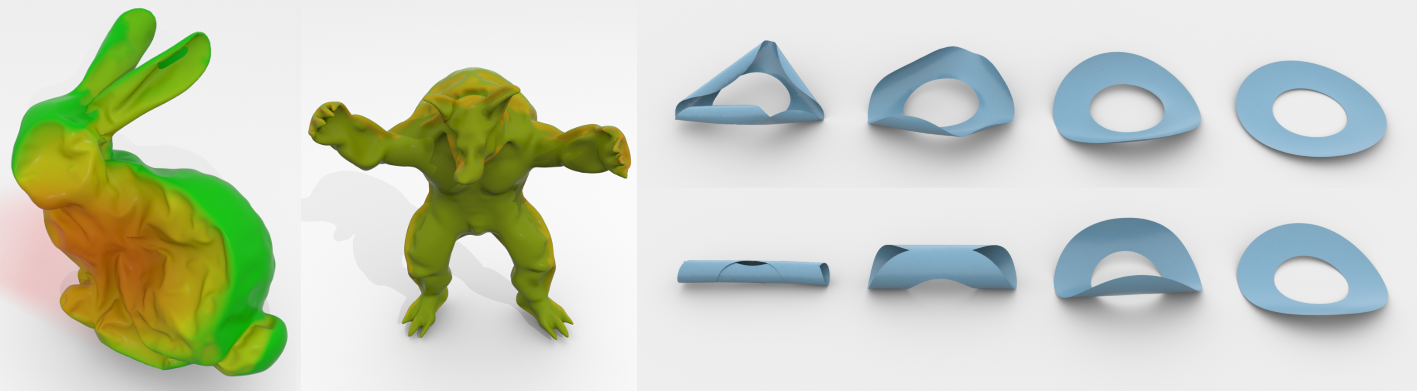
\includegraphics[width=\textwidth]{teasernew.png}
  \caption{The geometry of thin materials often changes dramatically in response to heat and moisture. A plastic bunny and armadillo shrink in response to being heated (left). Colors on the surfaces indicate temperature (redder is hotter). Moist paper annuli curl up as they dry, and the amount and shape of curling is based on the paper's thickness and whether or not the paper's fibers are randomly or consistently oriented (right).}
\end{teaserfigure}

%% Processes all of the front-end information and starts the body of the work.
\maketitle

\section{Introduction}
Consider the wrinkling and curling of a drying leaf. The drying process corresponds to water evaporating from the internal cells, so that the tissue contracts in volume. This process typically happens differentially, due to having one side exposed to the sun, or having boundaries farther away from the veins than interior, leading to non-uniform curvature and curling of the leaf ~\cite{Xiao2011, Jeong2013}. Related phenomena are the swelling and wrinkling of paper when exposed to water, such as when coffee is spilled on a notebook page, or the wrinkling and shrinking of plastic when heated. Although the physical mechanisms in these examples are different (shrinking of cells vs swelling of fibers vs contraction of polymers) the \emph{effect} on the objects is the same: the intrinsic geometry of the thin objects change over time in response to dynamic changes in the environment. 

In addition to growth, wrinkling, and swelling, other phenomena involving the same physics include burning of thin objects, especially those made of curved or composite materials; wilting of flowers and dynamic response of plants to like light/moisture/etc; changes and wrinkling in skin due to aging, moisture, creams; shrinking and subsequent wrinkling of clothes; warping of wood due to one-sided heating; etc. There is also increasing excitement about manufacturing processes based on differential or inhomogeneous growth, that require precise control over the material's rest geometry. Examples include water printers that induces paper bending~\cite{Guberan2012}, two-layer structures consisting of plastic printed on canvas under tension~\cite{Perez2017}, the various works of Nervous Systems~\cite{NervousSystems}, fabrication using networks of filaments that stretch anisotropically when moistened, etc. Exploiting these technologies requires solving challenging inverse problems, with reliable methods for solving \emph{forward} problems an essential first step. 

Of course, one could capture all of these phenomena by modeling elastic volumes explicitly using tetrahedral or hexahedral elements, and tracking the change in moisture, heat, etc within each element. However, such a volumetric model is computationally expensive, and unnecessary: structures that are thin relative to their surface diameter ought to be able to benefit form a reduced elastic shell model, augmented to track and account for dynamic changes in the environmental stimulus throughout the shell volume. Yet previous methods studying phenomena such as burning of paper~\cite{Liu2009}, drying of leaves~\cite{Jeong2013}, cooking pasta~\cite{Wang2017}, etc, have used either ad-hoc application-specific shell models, or volumetric finite elements, to account for intrinsic geometric changes. Our goal instead is to provide a principled low-order simulation methodology for such systems. This goal can be broken into two connected challenges: to simulate the object's elastic response to changes in its intrinsic geometry, and to model its intrinsic geometry changes in response to environmental stimuli. In this work we addressed both, generating a numerical method that allows researchers studying growth and related phenomena to plug in any realistic model and parameter set, and reap a working simulation.

\paragraph{Contribution} We present a unified low-order discrete shell model tailored to simulating non-uniform, anisotropic, differential growing and shrinking of thin shells. This model is needed for simulating real-world thin materials whose geometry changes in response to stimuli such as heat, moisture, and growth. In contrast to previous methods for simulating such phenomena, our formulation builds on discrete geometric shell theory and supports arbitrary rest curvature and strain, and physical settings such as thickness and Lam\'{e} parameters. We couple our shell model to a simple formulation of moisture and temperature diffusion in both the lateral and thickness directions, which takes into account anisotropy of the material grain. In a series of experiments, we show that our model successfully predicts the qualitative behavior of thin shells undergoing complex, dynamic deformations due to material expansion or contraction, such as occurs when paper is moistened or thin plastic melts.

\subsection{Related Work}
\paragraph{Simulating Burning/Melting/Swelling} Several papers look at related problems, such as evolving the boundary of a burning or melting solid, without incorporating curling/wrinkling and other elastic deformations of the solid. Melek and Keyser~\shortcite{Melek2003,Melek2005} simulate pyrolysis and heat diffusion of burning objects, but do not consider their elastic deformation. Losasso et al~\shortcite{Losasso2006} proposed tracking of the burning boundary of thin shells using an adaptive level set on the shell. Some of the deformation can be qualitatively approximated by mapping physical quantities like heat and moisture to cells of a coarse grid around the object, deforming the cage, and mapping the deformation back onto the shell (as in Free Form Deformation); this approach was proposed by Melek and Keyser~\shortcite{Melek2007} and adopted by Liu et al~\shortcite{Liu2009}.

Steps towards a more principled elastic model include the use of a mass-spring network to represent the shell, with update rules for how spring rest lengths should change due to physical processes in the shell. Such rules are simplest to formulate in the case where growth or shrinkage is uniform through the shell thickness, and the shell can be represented using a single spring layer; Larboulette et al~\shortcite{Larboulette2013} present such a rule, which includes handling of the \emph{machine direction} of paper: a bias in the orientation of the fibers composing the paper which causes the paper to swell anisotropically. We adopt this parameter in our material model. 

Most similar to our work is the method of Jeong et al~\shortcite{Jeong2011,Jeong2013}, which uses a \emph{bilayer} of springs (a triangle mesh and its circumcentric dual, offset a distance from the primal mesh) to represent the shell. The bilayer allows the method to capture \emph{differential} growth due to gradients in moisture concentration across the thickness of leaves, leading to visually impressive simulations of leaves curling as they dry. Our work is based on the same fundamental idea (representing the shell using a rest strain that varies linearly through the thickness) but couched in the machinery of differential geometry; our formulation allows us to easily incorporate non-zero rest curvature, machine direction, and a physical material model. Also somewhat related are the \emph{CurveUps} of Guseinov et al~\shortcite{Guseinov2017}, which induce rest curvature in shells by embedding rigid pieces within a pre-stressed substrate.

\paragraph{Mechanics of Shells}
The mathematics underpinning the physics of thin shells is a venerable topic: Ciarlet's book~\shortcite{Ciarlet2000} on elasticity as applied to shells offers a thorough overview. Our work is based on the common \emph{Kirchhoff-Love} assumption that the shell does not undergo any transverse shear; i.e., that the shell volume is foliated by normal offsets of the shell's \emph{midsurface}. The problem of studying deformation of the 3D shell volume then reduces to that of deformation of a 2D surface, and tools from Riemannian geometry can be applied~\cite{Simo1989}.\footnote{We adopt the so-called ``intrinsic'' view~\cite{Neff2004} that shells can be understood in terms of Kirchhoff-Love and geometric principles, as this view allows us to easily discretize shell physics by leveraging discrete differential geometry, but we note in passing that the validity of the Kirchhoff-Love assumption, and of reduced shell models in general, remains unsettled, and the literature documents numerous alternative shell theories.} One key property of the shells we want to simulate is that they are \emph{non-Euclidean}: they do not have a rest (strain-free) state that is realizable in three-dimensional space. Non-Euclidean shells have received substantial attention recently in the physics community~\cite{Klein2007,Kim2012}, thanks to their potential applications in fabrication and robotics, and their connection to biological growth; physicists such as Sharon, Efrati, and Ben Amar~\cite{Goriely2005, Dervaux2008,Efrati2009,Sharon2010} pioneered the study of shell mechanics in this setting.

For the sake of being self-contained, we briefly review the geometric foundations of shell mechanics in Section \ref{sec:continuous}.

\paragraph{Computational Modeling of Thin Shells} 
Thin shells first caught the interest of the graphics community in the context of simulating cloth~\cite{Baraff1998,Bridson2002}. These early methods tended to focus on thin \emph{plates}, i.e. shells that have a flat rest configuration, and formulate shell dynamics in terms of either hinge-based bending energies~\cite{Sullivan2008,Tamstorf2013} or the insight that the bending energy can be written in terms of the intrinsic Laplace-Beltrami operator applied to the shell's embedding function~\cite{Bobenko2005,Bergou2006,Wardetzky2007}. 

\begin{wrapfigure}{r}{1.6in}
\centering
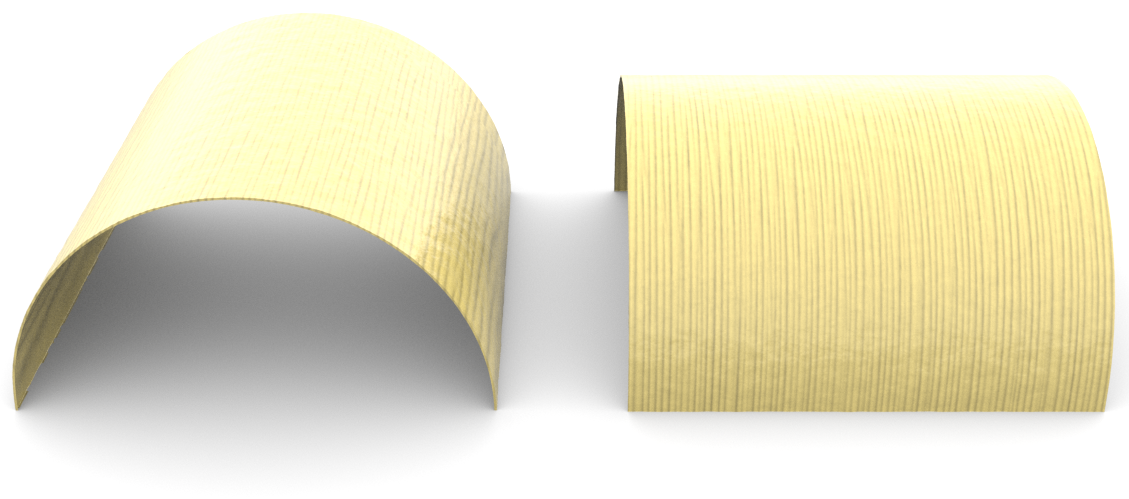
\includegraphics[width=1.6in]{cyls.png}
\label{fig:cyls}
\end{wrapfigure}
Grinspun et al~\shortcite{Grinspun2003} introduced to graphics the simulation of shells with non-zero rest curvature. Their formulation is based on \emph{differences of squared mean curvature}, leading to a simple and easy-to-discretize bending energy. This model is physically suspect, however: consider a half-cylinder at rest when curled around the $x$-axis. Unbend the shell and re-bend it around the $y$-axis; the deformed configuration's strain cannot be captured by looking at mean curvature alone, as it is pointwise identical to the mean curvature of the rest configuration (see inset). Complete support for rest curvature therefore requires a bending energy that incorporates full information about the extrinsic deformation of the shell~\cite{Grinspun2006}. One such discrete energy is described in Weischedel's work on discrete Cosserat shells~\shortcite{Weischedel2012}; our exposition is modeled closely on hers, though we make different modeling choices (we use an intrinsic rather than Cosserat shell model, and require more flexible handling of the shell rest geometry).

A popular alternative to Grinspun et al.'s bending formulation based on the mid-edge shape operator is to use a triangle-averaged shape operator proposed by Gingold et al.~\shortcite{Gingold2004}, which expresses bending energy of a triangle in terms of the hinge angles of each of its three edges. Gingold et al. demonstrate how plasticity can be implemented by maintaining and dynamically updating ``rest'' values of the hinge angles, and also propose a simple method for simulating thin shell fracture. Although Grinspun et al. raised concerns about the consistency of this averaged shape operator, it is simple to implement and has been adopted in thin shell simulation frameworks like ArcSim~\cite{Narain2013}. We briefly discuss how Gingold et al.'s operator might be adapted for non-Euclidean rest geometry in Section~\ref{sec:gingold}.

Higher-order methods for simulating shells (including with NURBS or subdivision elements) are common in computational mechanics and isogeometric analysis~\cite{Batoz1980,Bathe1983,Cirak2000,Kiendl2009,Benson2010,Bandara2018} and have also been proposed for computer graphics~\cite{Wawrzinek2011} and growing shells~\cite{Vetter13}. High-order methods have some obvious advantages (better convergence behavior in the thin limit, continuous surface normals) at the cost of additional computation and complexity, especially when handling contact.

In this paper, we ignore the problem of mesh tessellation, or of adapting the mesh in response to either large deflections or large amounts of growth; such remeshing is an important component of a practical shell simulation but orthogonal to our focus on shell dynamics. An existing tool such as ArcSim~\cite{Narain2012}, which incorporates a method of adaptive remeshing while avoiding significant popping artifacts, could easily be adopted in our framework if desired.

\begin{figure}
\begin{tikzpicture}
    \draw (0, 0) node[inner sep=0] {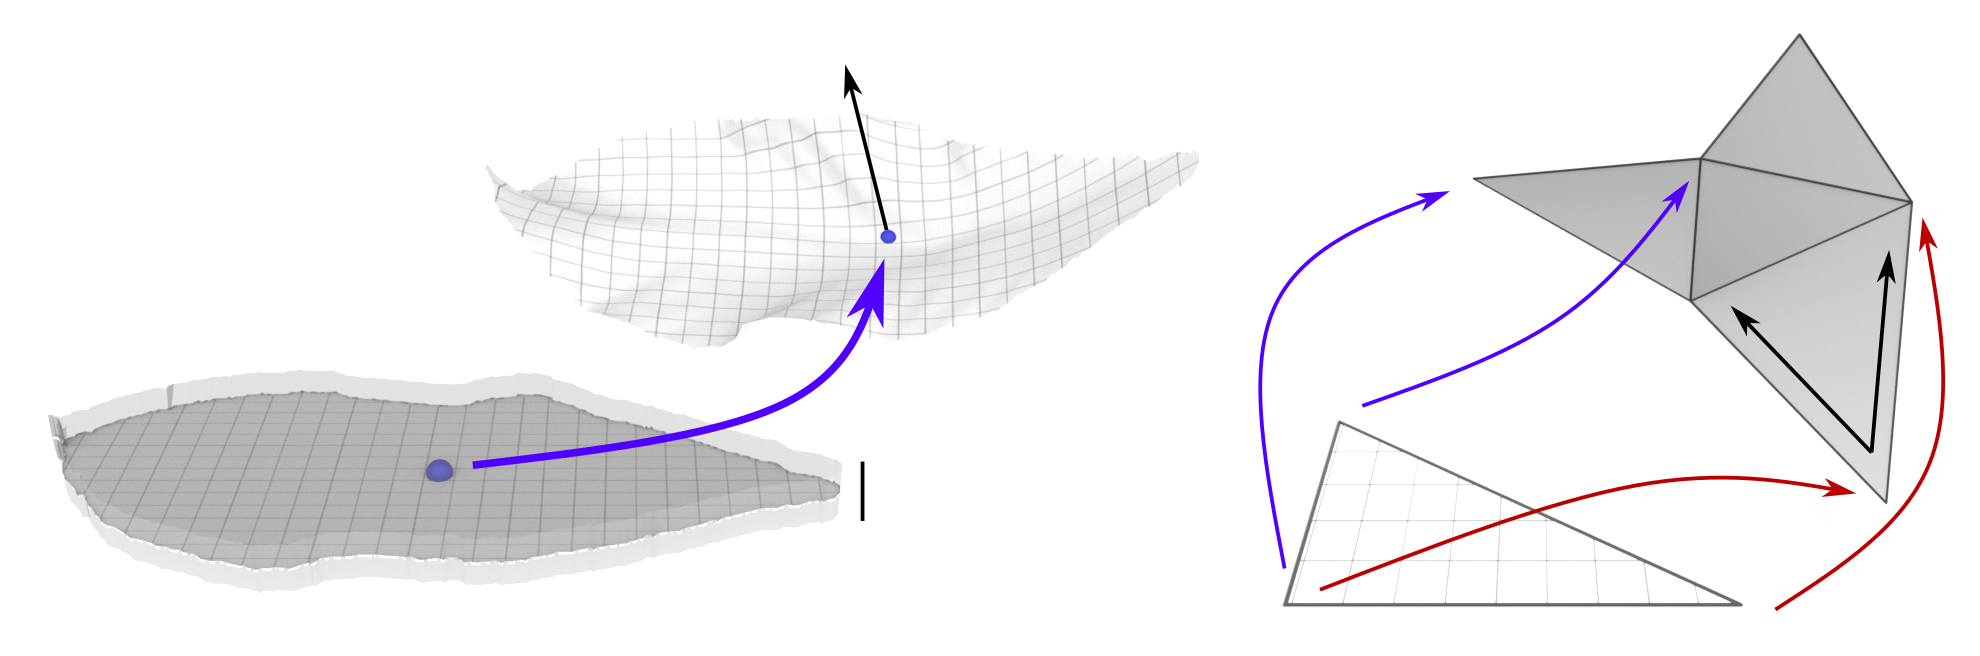
\includegraphics[width=\columnwidth]{technical.png}};
    \draw (-3, -0.7) node {$\Omega$};
    \draw (-0.4, -0.73) node {$h$};
    \draw (-0.1, -0.18) node {$\br(x,y)$};
    \draw (2, 0.8) node {$v_0$};
    \draw (-0.4, 1.1) node {$\hn$};
    \draw (3, 0.85) node {$v_1$};
    \draw (2.6, 0.6) node {$\bff_{021}$};
    \draw (3, -0.05) node {$v_2$};
    \draw (3.5, 0.06) node {$\scriptsize{u_1}$};
    \draw (3.8, 0.4) node {$\scriptsize{u_2}$};
    \draw (4.2, 0.6) node {$v_4$};
    \draw (4.2, -0.8) node {$v_3$};
    \draw (1.8, -0.8) node {$\mathcal{T}$};
    \draw (0.9, -1.4) node {$(0,0)$};
    \draw (1.5, -.2) node {$(0,1)$};
    \draw (3.5, -1.4) node {$(1,0)$};
\end{tikzpicture}
\caption{Left: the volumetric shell is parameterized by a slab $\Omega \times [-h/2,-h/2]$ around a region $\Omega$ in the plane. $\br$ maps $\Omega$ to the shell midsurface. Right: we parameterize all triangles of discrete shells by a single canonical triangle $\mathcal{T}$. We express all face-based quantities in the face's local barycentric coordinate system $(u_1,u_2)$, which is not consistent across faces.}
\label{fig:technical}
\end{figure}
\section{Continuous Formulation} \label{sec:continuous}
Before describing our discretization of shells, we briefly review the formulation in the continuous setting, as this formulation will guide our discretization. 

\paragraph{Shell Geometry} We can represent shells $S\subset \mathbb{R}^3$ of thickness $h$ by a parameter domain $\Omega$ in the plane and an embedding $\phi\colon \Omega\times [-h/2, h/2]\to\mathbb{R}^3$ with $S$ the image of $\phi$ (see Figure~\ref{fig:technical}). The Kirchhoff-Love assumption allows us to represent the entire shell volume only in terms of the shell's \emph{midsurface} $\br\colon\Omega\to\mathbb{R}^3$. In other words,
$$\phi(x,y,z) = \br(x,y) + z\hn(x,y)$$
where $\hn = (\br_x \times \br_y)/\|\br_x \times \br_y\|$ is the midsurface normal. The metric $\bg$ on the slab $\Omega \times [-h/2,h/2]$, pulled back from $\mathbb{R}^3$, can be expressed in terms of the geometry of the midsurface:
\begin{equation}
\bg = \left[\begin{array}{cc}\ba - 2z\bb + z^2 \bc & 0\\0 & 1\end{array}\right],\label{eq:offset}
\end{equation}
where
$$\ba = d\br^Td\br \quad \bb = -d\br^Td\hn \quad \bc = d\hn^Td\hn$$
are the classical first, second, and third fundamental forms of the surface $\br$.

Oftentimes, the parameterization domain of a thin shell is assumed to be also the rest state of the shell, so that the strain in the material of the shell can be determined directly from looking at $\bg$. We cannot assume this: consider for instance a piece of paper whose center has been moistened by spilled coffee. The fibers in the coffee stain stretch; since they are confined by the surrounding non-wet region of the paper, the paper cannot globally stretch in such a way that both the wet and dry regions of the paper are simultaneously at rest. Instead, the paper will \emph{buckle} out of plane, into a shape that compromises between relaxing the in-plane (stretching) strain and the introduced bending strain. At this point the paper's rest state is \emph{non-Euclidean}---it is impossible to find any embedding of the paper into $\mathbb{R}^3$ that is entirely strain-free.

We therefore record the rest state of the shell using a \emph{rest metric} $\bar\bg(x,y,z)$~\cite{Efrati2009}.\footnote{Here and throughout the paper, we use an overbar to denote quantities associated to the shell rest state.} Since our model is tailored to simulating differential in-plane swelling or shrinking across the thickness of the shell, we make the simplifying assumption that this rest metric is linear in the thickness direction:
$$\bar\bg(x,y,z) = \left[\begin{array}{cc}\bar\ba(x,y) - 2z\bar\bb(x,y) & 0\\0 & 1\end{array}\right].$$
A shell that begins a simulation at rest will simply have $\bar\ba = \ba^0$ and $\bar\bb = \bb^0$, where $\ba^0$ and $\bb^0$ are the values of $\ba$ and $\bb$ at the start of the simulation, respectively; this setup is a special case of a shell which has a rest state specified by a ``rest surface'' $\bar\br$ that is isometrically embeddable in $\mathbb{R}^3$, in which case $\bar\ba$ and $\bar\bb$ are the first and second fundamental forms of that rest surface. Therefore $\bar\ba$ and $\bar\bb$ can be thought of as representing the ``rest metric'' and ``rest curvature'' of the shell's midsurface, respectively.\footnote{We stress, though, that these labels are to provide intuition only---$\bar\ba$ and $\bar\bb$ must not, and generally will not, satisfy usual relationships from differential geometry such as the Gauss-Codazzi-Mainardi equations.}

\begin{figure*}[h]
  \centering
  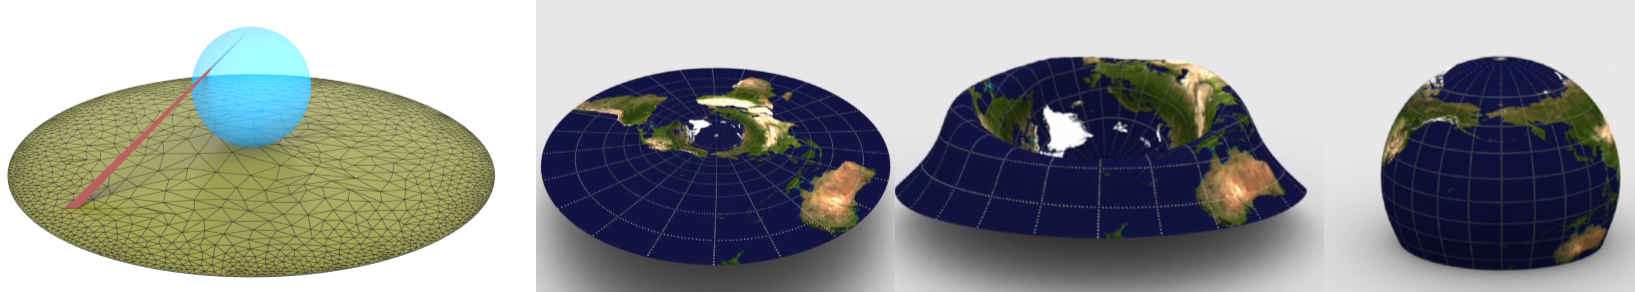
\includegraphics[width=\textwidth]{ContractingSphere.png}
  \caption{Stereographic projecion of the disk into the plane yields a conformal parameterization of one by the other (left); we set $\bar\bb=0$ and $\bar\ba$ to this conformal metric, and simulate the disk dynamics as it relaxes to equilibrium by adopting a spherical shape (right).}
  \label{ContractingSphere}
\end{figure*}

To summarize, our parameterization of thin shells involves the following kinematic elements:
\begin{itemize}
\item a thickness $h$ and parameterization domain $\Omega\subset\mathbb{R}^2$, both of which are fixed over the course of the simulation;
\item an embedding $\br:\Omega\to\mathbb{R}^3$ representing the shell midsurface's ``current'' or ``deformed'' geometry, and which evolves over time. From this embedding, the current midsurface normals $\hn$ can be calculated, and thus $\br$ provides the embedding of the full shell volume $\phi$, as well as the midsurface fundamental forms;
\item a rest metric $\bar\bg$, parameterized by the pair of tensor fields $\bar\ba, \bar\bb$ over $\Omega$, respectively. These might also evolve over time, due to changes in the shell rest state via expansion or contraction.
\end{itemize}

\subsection{Shell Dynamics}
Motivated by the common observation that a sufficiently thin shell bends much more readily than it will stretch, we assume that the shell's deformation involves \emph{large rotations} but only small in-plane strain of the midsurface: $\|\bar\ba^{-1}\ba- \Id\|_{\infty} < h.$ We also assume that the shell's material is uniform and isotropic. The simplest constitutive law consistent with these assumptions is the St. Venant-Kirchhoff material model\footnote{The neo-Hookean material model is also popular in computer graphics and could be used instead, although there is little benefit to doing so when simulating thin shells since strains are typically small.} together with Green strain; it can be shown~(see e.g. Weischedel~\shortcite{Weischedel2012}) that these choices yield an elastic energy density~(the \emph{Koiter shell model}) that can be approximated up to $O(h^4)$ by
\begin{equation}
W(x,y) = \left(\frac{h}{4} \|\bar\ba^{-1}\ba - \Id\|^2_{SV} + \frac{h^3}{12}\|\bar\ba^{-1}(\bb-\bar\bb)\|^2_{SV}\right)\sqrt{\det \bar\ba} \label{eq:koiter}
\end{equation}
where $\|\|_{SV}$ is the ``St. Venant-Kirchhoff norm''~\cite{Weischedel2012}
$$\|M\|_{SV} = \frac{\alpha}{2}\tr^2 M + \beta \tr\left(M^2\right),$$
for material parameters $\alpha, \beta$. In terms of the Young's modulus $E$ and Poisson's ratio $\nu$,
$$\alpha = \frac{E\nu}{1-\nu^2}, \quad \beta = \frac{E}{2(1+\nu)}.$$ % wim: check Ciarlet, An Introduction to Shell Theory - last equation of section 2.5 (p39): in 2D theory, the prefactor for the first term is actually ~ lambda mu / (lambda + 2 mu), where lambda and mu are the 3D Lame constants (what you had for alpha, beta originally). Working this out gives the correct definition for alpha, beta - though it is not correct to call them Lame parameters (sometimes they're called 2D Lame parameters).  Also see our PNAS paper on growing surfaces, SI : with these definitions, we correctly reproduce the Foppl-von Karman equations after simplifying for small deformations. Also see Efrati's paper deriving non-Euclidean elasticity, equation 3.6 --> definition of A^{alpha,beta,gamma,delta} is consistent with all this. So I still think Weischedel is wrong here to use the 3D Lame constants directly.
We thus have a formulation of kinetic energy and potential energy
$$T[\dot\br] = \int_{\Omega} h\rho\|\dot\br\|^2 \sqrt{\det\bar\ba}\,dxdy, \quad V[\br] = \int_{\Omega} W(x,y)\,dxdy,$$
for volumetric density $\rho$, to which additional external energies and forces (gravity, constraint forces, etc) can be added to yield equations of motion via the usual principle of least action.

\section{Discretization} \label{sec:discretization}
We approximate the midsurface $\br$ with a triangle mesh $(V,E,F)$; the positions of the vertices $\bv = [\bv_1, \bv_2\,\ldots]$ take the place of the embedding function $\br$. The general strategy we will use is to assume that $\ba$ and $\bb$, as well as their rest counterparts $\bar\ba$ and $\bar\bb$, are constant over each face of the triangle mesh; it will then be straightforward to write down a discrete analogue of the Koiter elastic energy density in Equation~\eqref{eq:koiter}. 

\paragraph{Discrete Shell Model} As in the continuous setting, the discrete shell does not necessarily have a rest state embeddable as a mesh in $\mathbb{R}^3$, making it impossible to parameterize the deformed configuration of the shell in terms of the rest configuration; additionally we do not want to assume (or compute) a global parameterization of the midsurface. Instead, we independently parameterize each triangle in its own barycentric coordinates (see Figure~\ref{fig:technical}). Let $\bff_{ijk}$ be a face in $F$ containing the vertices $\bv_i$, $\bv_j$, $\bv_k$, and denote by $\fT$ the canonical unit triangle with vertices $(0,0)$, $(1,0)$, $(0,1)$. Then locally the face $\bff_{ijk}$ is embedded by the affine function
$$\br_{ijk}:\fT\to\mathbb{R}^3, \quad \br_{ijk}(u_1,u_2) = \bv_i + u_1(\bv_j-\bv_i)+u_2(\bv_k-\bv_i);$$
under this embedding, the Euclidean metric on face $\bff_{ijk}$ pulls back to the first fundamental form
$$\ba_{ijk} = \left[\begin{array}{cc} \|\bv_j-\bv_i\|^2 & (\bv_j-\bv_i)\cdot(\bv_k-\bv_i)\\
(\bv_j-\bv_i)\cdot(\bv_k-\bv_i) & \|\bv_k-\bv_i\|^2\end{array}\right]$$
on $\fT$. If we are given an explicit rest configuration $\bar\bv_i$ of the shell, we can compute the rest first fundamental form $\bar\ba_{ijk}$ analogously; or alternatively we can set $\bar\ba_{ijk}$ to any desired symmetric positive-definite $2\times 2$ matrix. Notice that any such matrix corresponds to some choice of ``rest lengths'' for the edges of face $\bff_{ijk}$ that obey the triangle inequality, but that two faces sharing a common edge do not necessarily agree about that length. 

These discrete fundamental forms are enough to discretize the stretching term in Equation~\eqref{eq:koiter}: each face contributes a term 
{\scriptsize
$$\int_{\fT} \frac{h}{4} \|\bar\ba_{ijk}^{-1}\ba_{ijk} - \Id\|^2_{SV}\sqrt{\det{\bar\ba_{ijk}}} = \frac{h}{8} \|\bar\ba_{ijk}^{-1}\ba_{ijk} - \Id\|^2_{SV}\sqrt{\det{\bar\ba_{ijk}}},$$
}%
where the division by two is due to the canonical triangle $\mathcal{T}$ having area $\frac{1}{2}$. This energy is quartic in the positions of the mesh vertices, and is exactly the energy of constant-strain triangle stretching elements commonly used in cloth simulation. 

For the bending term, we also need a discretization of the second fundamental form. Here there is a significant departure between the smooth theory and the discrete approximation: we would like to apply the Kirchhoff-Love principle to extrude the mid-surface into a shell volume, but unfortunately normal offsets of triangle meshes are no longer guaranteed to be triangle meshes (or even piecewise-affine). One can instead look at weaker notions of mesh parallellity~\cite{Bobenko2010}:
\begin{itemize}
\item \emph{vertex offsets} require choosing a normal at each mesh vertex (itself a problem without an obvious solution), and moving each vertex a constant distance along this normal usually does not result in faces parallel to the original faces;
\item \emph{edge offsets} likewise do not guarantee parallel faces;
\item \emph{face offsets} are not conforming: moving each of the faces neighboring a vertex of valence four or higher in their normal directions yields new faces that are not guaranteed to still intersect at a common point.
\end{itemize}

While there is no perfect choice, we use the discretization that arises from edge parallelity, leading to the so-called ``mid-edge'' discretization of the second fundamental form~\cite{Grinspun2006,Weischedel2012}. This approach has several advantages: first, computing the edge offsets of a face requires knowing only the geometry of that face and its three edge neighbors, leading to a compact and constant-size discrete stencil for computing the discrete second fundamental form. By contrast, vertex offsets lead to stencils that vary depending on vertex valence. Moreover, the mid-edge formulation is significantly more robust to triangle inversion artifacts. Unlike in a face-offset-based approach, it also allows us to discretize rest second fundamental forms in the same place as the first fundamental forms, on the mesh faces.

Let $\be_i$ denote the edge opposite vertex $i$ on face $\bff_{ijk}$, and define the \emph{mid-edge normal} $\hn_i$ by:
\begin{itemize}
\item the face normal $\frac{(\bv_j-\bv_i)\times (\bv_k-\bv_i)}{\|(\bv_j-\bv_i)\times (\bv_k-\bv_i)\|}$, if $\be_i$ is a boundary edge;
\item the mean of the face normals of the two faces incident on $\be_i$, otherwise.
\end{itemize}

Let $\bff_{ijk}^{\epsilon}$ denote the triangle formed by offsetting all of $\bff_{ijk}$'s edges in their mid-edge normal direction by a distance $\epsilon$, and let $\ba^{\epsilon}_{ijk}$ be the discrete first fundamental form of that offset triangle. Then the discrete second fundamental form $\bb$ can be defined, by analogy to Equation~\eqref{eq:offset}, as the first-order correction
$$\ba^{\epsilon}_{ijk} = \ba_{ijk} - 2\epsilon \bb_{ijk} + O(\epsilon^2),$$
leading to the formula
$$\bb_{ijk} = \frac{1}{2}\left[\begin{array}{cc}(\hn_i-\hn_j)\cdot(\bv_i-\bv_j) & (\hn_i-\hn_j)\cdot(\bv_i-\bv_k) \\ (\hn_i-\hn_k)\cdot(\bv_i-\bv_j) & (\hn_i-\hn_k)\cdot(\bv_i-\bv_k)\end{array}\right].$$
(Alternatively, this formula can be derived by discretizing the relation $\bb = -d\br^Td\hn$ using divided differences). Although it may not appear so at first, the matrix $\bb_{ijk}$ is always symmetric (since each mid-edge normal is orthogonal to that edge); it is not in general positive-definite.\footnote{As observed by Grinspun et al~\shortcite{Grinspun2006}, the \emph{shape operator} $d\hn$ in the continuous setting always maps tangent vectors to tangent vectors, whereas in the discrete setting the finite difference of mid-edge normals is not always parallel to the mesh triangle. This discrepancy is a consequence of the failure of edge-offset meshes to also be face-offsets. Corrections to the shape operator have been proposed to remedy this quirk, though we found them unnecessary (and in any case, any components of $d\hn$ that lie orthogonal to the face are annihilated when forming the second fundamental form $-d\br^Td\hn$).} We represent the rest second fundamental form $\bar\bb_{ijk}$ by an arbitrary symmetric $2\times 2$ matrix assigned to each face.

\begin{figure}
\centering
    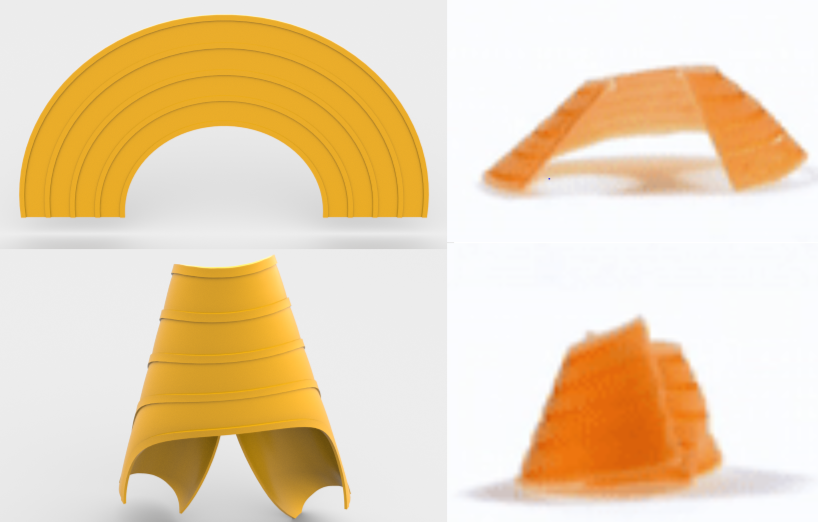
\includegraphics[width=0.5\textwidth]{PastaCombined.png}
\caption{We simulate one of Wang et al.'s~\shortcite{Wang2017} shape-changing pasta designs, consisting of a half-annulus decorated with concentric rings which are both thicker (and thus more bending-resistant) and less porous than the surronding material. Our simulation predicts qualitatively identical curling behavior of the pasta as both the physical experiment and volumetric FEM simulation conducted by Wang et al. Top-left: the initial geometry, showing the thickened concentric ribs. Bottom-left: our simulated result. Right: photographs of Wang et al's experimental results, at different stages of swelling. Photographs reproduced with permission.}
\label{fig:pasta}
\end{figure}

\paragraph{Choosing Rest Fundamental Forms}
Depending on the mechanism for growth being simulated, there are several choices for how to set and update $\bar\ba$ and $\bar\bb$:
\begin{itemize}
\item \textbf{No Growth}: A classic shell, whose rest state is fixed, simply has $\bar\ba=\ba^0$ and $\bar\bb=\bb^0$, where $\ba^0$ denotes the first fundamental form induced by $\bv^0$, the positions of the midsurface vertices at the beginning of the simulation. (And if the shell is pre-strained, $\bar\ba, \bar\bb$ can be adjusted appropriately).
\item \textbf{Pullback Forms}: In the case where the shell's initial configuration is flat, it is natural to align it with a region of the $xy$ plane, and prescribe rest fundamental forms in Euclidean $(x,y)$ coordinates, instead of prescribing an $\bar\ba_{ijk}$ in the barycentric coordinates of each triangle. Let $\bar\ba^{xy}$ and $\bar\bb^{xy}$ be such prescribed forms; these can be sampled on each triangle $\bff_{ijk}$'s centroid and pulled back to the triangle's parameterization domain to give
$$\bar\ba = T^T\bar\ba^{xy}(\xi)T, \qquad  \bar\bb = T^T\bar\bb^{xy}(\xi)T$$
in barycentric coordinates, where
$$T = \left[\begin{array}{cc}\bv^0_{j} - \bv^0_{i} & \bv^0_{k}-\bv^0_{i}\end{array}\right]$$
maps from vectors in the barycentric coordinates of $\bff_{ijk}$ to Euclidean space, and $\xi = \frac{1}{3}(\bv_i+\bv_j+\bv_k)$ is the face centroid.

\item \textbf{Isotropic Growth}: In many cases growth is isotropic and uniform through the thickness of the shell (for instance, when plastic shrinks in response to heat, or biological tissue grows through cell division). In this case 
$$\bar\ba = e^{2s_{ijk}}\ba^0, \qquad \bar\bb = \bb^0$$
for a per-face conformal factor $s$ encoding the amount of growth (or shrinking, if negative).

\item \textbf{Linear Differential Swelling}: Porous materials like paper swell when moistened, and differences in water concentration through the thickness of a thin shell can induce metric frustration and buckling. This mechanism is responsible for the buckling of paper when wet, and the curling of leaves as they dry. 

We model this swelling mechanism by assuming that the amount of moisture varies linearly in the thickness direction of the shell, and represent the percentage of additional moisture present in the material at the top and bottom of the shell by two scalars $m^+_{i}, m^-_{i}\in \mathbb{R}$ at each vertex $\bv_i$. We average these values to compute a moisture content $m^{\pm}_{ijk}$ per face $\bff_{ijk}$. The additional water content induces swelling, which changes the rest geometry; assuming a linear relationship between rest length and moisture concentration~\cite{iggesund1993paperboard}, we can write the rest metric of the volumetric shell as
$$\bar\bg = \left[\begin{array}{cc} \bar\bg^-\left(\frac{1}{2}-\frac{z}{h}\right) + \bar\bg^+\left(\frac{1}{2}+\frac{z}{h}\right) & 0\\0 & 1\end{array}\right].$$
Here $\bar\bg^+$ and $\bar\bg^-$ are the metric on the top and bottom of the shell,
\begin{align*}
\bar\bg^+ &= (1 + m^+\mu)^2(\ba^0 - h \bb^0)\\
\bar\bg^- &= (1+m^-\mu)^2(\ba^0 + h \bb^0),
\end{align*}
for moisture expansion coefficient $\mu$. Then
{\scriptsize
\begin{align*}
\bar\ba &= \frac{(1+m^+\mu)^2 + (1+m^-\mu)^2}{2}\ba^0 + h\frac{(1+m^-\mu)^2 - (1+m^+\mu)^2}{2}\bb^0\\
\bar\bb &= \frac{(1+m^-\mu)^2 - (1+m^+\mu)^2}{2h}\ba^0 + \frac{(1+m^+\mu)^2 + (1+m^-\mu)^2}{2}\bb^0.
\end{align*}
}%

\item\textbf{Piecewise Constant Differential Swelling} Instead of a linear moisture gradient through the thickness, in some cases it is more appropriate to model a piecewise constant moisture profile, such as when modeling bilayers with different material properties. For example, Wang et al~\shortcite{Wang2017} fabricate exotic pasta geometries by cooking pasta composed of two layers of different porosity. van Rees et al~\shortcite{vanRees17} showed that a bilayer of thickness $h$ with piecewise-constant rest metric
$$\bar\bg(z) = \left[\begin{array}{cc}\begin{cases}\bar\bg^+, z>0\\ \bar\bg^-, z<0\end{cases} & 0\\ 0 & 1\end{array}\right]$$
is \emph{energetically equivalent} to a shell with linearly-varying metric
$$\bar\ba = \frac{\bg^+ +\bg^-}{2}, \qquad \bar\bb = \frac{3}{4h}(\bg^--\bg^+);$$
thus the desired piecewise-constant metric taking into account moisture-induced swelling is
\begin{align*}
\bar\bg^+ &= (1 + m^+\mu^+)^2\left(\ba^0 - \frac{2}{3}h \bb^0\right)\\
 \bar\bg^- &= (1+m^-\mu^-)^2\left(\ba^0 + \frac{2}{3}h \bb^0\right),
 \end{align*}
where $\mu^+$ and $\mu^-$ encode the differing moisture-length relationship in the two layers. Converting this piecewise-constant metric back into the equivalent linear metric gives
{\scriptsize
\begin{align*}
\bar\ba &= \frac{(1+m^+\mu^+)^2 + (1+m^-\mu^-)^2}{2}\ba^0 + h\frac{(1+m^-\mu^-)^2 - (1+m^+\mu^+)^2}{3}\bb^0\\
\bar\bb &= 3\frac{(1+m^-\mu^-)^2 - (1+m^+\mu^+)^2}{4h}\ba^0 + \frac{(1+m^+\mu^+)^2 + (1+m^-\mu^-)^2}{2}\bb^0.
\end{align*}
}%

\item\textbf{Linear Differential Swelling with Machine Direction} In paper, leaves, and other materials composed of microscopic fibers, swelling induced by moisture is \emph{anisotropic}, since fibers swell more in their circumferential than axial direction. We can model this behavior by storing a \emph{machine direction} $\bd_{ijk}$ per triangle face; this direction, a vector in the barycentric coordinates of the triangle, is the direction in which the fibers are aligned. Given this direction, we can compute the intrinsically orthogonal direction $\bd_{ijk}^{\perp}$ (with $\bd_{ijk}^T \ba_{ijk}^0 \bd_{ijk}^{\perp} =0$), and impose different moisture-length constants $\mu$ and $\mu_{\perp}$ in the $\bd$ and $\bd^{\perp}$ directions, respectively. Then the desired rest metrics at the top and bottom of the shell are 
\begin{align*}
\bar\bg^+ &= T^T M^+ T^{-T} (\ba^0 - h \bb^0) T^{-1}M^+T,\\
\bar\bg^- &= T^T M^- T^{-T} (\ba^0 + h \bb^0) T^{-1}M^-T.
\end{align*}
where 
$$T = \left[\begin{array}{cc} \bd & \bd^{\perp}\end{array}\right]^{-1}$$
transforms from the triangle's barycentric coordinates to the $\bd,\bd^{\perp}$ coordinate system, and
$$M^{\pm} = \left[\begin{array}{cc}
(1 + m^{\pm}\mu) & 0\\0 & (1+m^{\pm} \mu_{\perp})\end{array}\right]$$
anisotropically stretches in the machine direction. As in the previous cases, the rest fundamental forms can be computed from these metrics using the formula
$$\bar\ba = \frac{\bar\bg^++\bar\bg^-}{2}, \qquad \bar\bb = \frac{\bar\bg^- - \bar\bg^+}{2h}.$$
\end{itemize}

\begin{figure*}[h]
  \centering
   \includegraphics[width=\textwidth]{BunnyandArmadilloNew.png}
  \caption{Time evolution of a plastic armadillo and a plastic bunny as they shrink when exposed to localized heating (red beam in the figure), where redder parts have higher temperature.}
  \label{fig:BunnyandArmadillo}
\end{figure*}

\paragraph{Elastic Energy} We can now write down the full elastic energy of the shell, in exact analogy to the Koiter energy:
{\scriptsize
$$E_{\mathrm{elastic}}(\bv) = \sum_{\bff_{ijk}\in F} \frac{\sqrt{\det \bar\ba_{ijk}}}{2}\Bigg(\frac{h}{4} \|\bar\ba_{ijk}^{-1}\ba_{ijk} - \Id\|^2_{SV} + \frac{h^3}{12}\|\bar\ba_{ijk}^{-1}(\bb_{ijk}-\bar\bb_{ijk})\|^2_{SV}\Bigg).$$
}%
It is worth making a few observations about this energy. First, the matrices $\ba$, $\bar\ba$, etc. are \emph{coordinate-dependent}: replacing the parameterization domain $\fT$, or even cyclically permuting the order of vertices around a face, would alter the values in the matrix. However, the generalized eigenvalues of $\ba-\bar\ba$ and $\bb-\bar\bb$ with respect to the inner product $\bar\ba$ are coordinate-\emph{independent}, as is the total energy. Perhaps the easiest way to see this fact is to note that these spectra measure the geometrically exact strain induced by an affine embedding of $\fT$, and so \emph{must} be independent of the coordinates chosen. Second, the terms of the form $\|\bar\ba^{-1}M\|^2_{SV}$ are sometimes instead written as $\|\bar\ba^{-1/2}M\bar\ba^{-1/2}\|^2_{SV}$, where $\bar\ba^{-1/2}$ is the unique positive-definite square root of $\bar\ba$. The two expressions are equivalent, since the spectrum of a product of matrices is invariant under cyclic permutation, but the form used above is slightly more convenient for computation. Finally, as a sanity check, observe that when $\bar\bb=0$ and the Poisson ratio $\nu=0$, the bending energy reduces to the square of mean curvature, as expected for thin plates.

\paragraph{Mass Matrix} Whether swelling or shrinking of the surface affects the mass of the surface depends on the mechanism: changes due to growth or moisture absorption/evaporation do change the mass, while plastic polymers contracting when exposed to heat do not. In cases where modeling the mass change is desired, the mass $\lambda_i$ of each vertex can be recomputed at a given instant in time by
$$\lambda_i = \sum_{\bff\sim \bv_i} \frac{\rho h}{3}\sqrt{\det \bar\ba_{\bff}}/2;$$
here the sum is over all faces $\bff$ incident to $\bv_i$ and yields the usual ``lumped'' or barycentric mass matrix $\Lambda$.\footnote{For absorption/evaporation, one might also want to model the fact that water has a different density than the shell material; we do not do so in our examples.}

\paragraph{Viscous Damping} Since the growth and swelling phenomena we want to simulate all take place at relatively long time scales, and paper and plastic are viscoelastic, a damping model is needed to dissipate the elastic waves in the material. We implement a simple Kelvin-Voigt damping model by including a damping potential
\begin{align*}
E_{\mathrm{damp}}(\bv, \bv^{\mathrm{prev}}) &= \frac{\eta}{E}\Delta t \sum_{\bff_{ijk}\in F} \frac{\sqrt{\det \bar\ba_{ijk}}}{2}\left(W_{\mathrm{s}} + W_{\mathrm{b}}\right)\\
W_{\mathrm{s}} &= \frac{h}{4} \left\|\left[\ba_{ijk}^{\mathrm{prev}}\right]^{-1}\frac{\ba_{ijk} - \ba_{ijk}^{\mathrm{prev}}}{\Delta t}\right\|^2_{SV}\\
W_{\mathrm{b}} &= \frac{h^3}{12}\left\|\left[\ba_{ijk}^{\mathrm{prev}}\right]^{-1}\frac{\bb_{ijk}-\bb_{ijk}^{\mathrm{prev}}}{\Delta t}\right\|^2_{SV}.
\end{align*}
where $\Delta t$ is the time step size, $\bv^{\mathrm{prev}}$ denotes the values of $\bv$ in the previous time step (and likewise for $\ba^{\mathrm{prev}}$, etc), and $\eta$ is a viscosity parameter.
\begin{table}[htb]
\begin{tabular}{lc}
Thickness &  $0.1\ \mathrm{mm}$\\
Young's Modulus $E$ & $2\times 10^9\ \mathrm{Pa}$\\
Poisson's Ratio $\nu$ & $0.3$\\
Density $\rho$ & $250\ \mathrm{kg/m^3}$\\
Viscosity $\eta$ & $5\times 10^{-13}\ \mathrm{Pa}\cdot\mathrm{s}$\\
Swelling constant $\mu$ & $0.0025$\\
Swelling constant $\mu^{\perp}$ & $0.001$
\end{tabular}
\caption{Table of reasonable physical parameters for ordinary paper.}
\label{tab:params}
\end{table}
\paragraph{Summary} In the discrete simulation, we track the following variables:
\begin{itemize} 
\item The configuration $\bv$ and configurational velocity $\dot\bv$. These vertex positions completely encode the kinematics of the discrete shell. 
\item Two matrices $\bar \ba$ and $\bar \bb$ per face in $F$, both symmetric, and with $\bar \ba$ positive-definite. These matrices store information about the rest state of the discrete shell, and may change over the course of the simulation. In most of our simulations, the mechanism for changes in the shell rest state is either change in temperature or absorption/evaporation of moisture; in this case we store two scalars $m^+$ and $m^-$ per vertex, indicating temperature/moisture concentration on the top and bottom boundary of the shell, and $\bar\ba$ and $\bar\bb$ are computed from these scalars, as described above.
\end{itemize}
In addition, we track a machine direction $\bd$ per face, which stays constant over the course of the simulation; finally Table~\ref{tab:params} lists the physical parameters and constants on which the simulation depends, as well as reasonable values of these parameters for the special case of ordinary paper. We use these default values in all experiments described below, unless specified otherwise.

\paragraph{Time Integration} We integrate the equations of motion using implicit Euler time integration:
\begin{align}
\Lambda\frac{\dot\bv^{i+1}-\dot\bv^{i}}{\Delta t} &= \bF\left(\bv^{i+1},\bv^i\right) \notag\\
\bv^{i+1} &= \bv^i + \Delta t \dot\bv^{i+1},\label{eq:implicit}
\end{align}
where superscripts denote the time step index, and the total force is given by
$$\bF\left(\bv^{i+1},\bv^i\right) = \bF_{\mathrm{ext}} - \nabla E_{\mathrm{elastic}}\left(\bv^{i+1}\right) - \nabla E_{\mathrm{damp}}\left(\bv^{i+1},\bv^i\right)$$
where $\bF_{\mathrm{ext}}$ encapsulates contact forces and external forces like gravity. Solving these equations requires computing first and second derivatives of the elastic energy; the derivatives of a triangle's stretching term depend only on the vertices of that triangle, whereas the derivatives of the bending term also depend on vertices of the neighboring three triangles (due to the dependence of $\bb$ on the mid-edge normals). The bending term in particular is somewhat unpleasant to differentiate due to its high degree of nonlinearity, and special cases that arise for triangles adjacent to the mesh boundary. We provide source code for calculating the derivatives in the supplemental material.

\section{Moisture Diffusion}
Moisture diffuses in both the thickness and in-plane directions of the shell, and from the environment into the shell. We assume that within the shell, moisture diffuses isotropically at a rate uniform throughout the shell, so that the percentage of additional moisture $m(x,y,z;t): \Omega\times [-h/2,h/2]\times \mathbb{R}\to\mathbb{R}$ obeys the diffusion equation
\begin{equation}
\frac{\partial m}{\partial t}(x,y,z) = \begin{cases}D\Delta_{\bg} m, & -h/2 < z < h/2\\
s(x,y,z), & z=\pm h/2,\end{cases} \label{eq:diffusion}
\end{equation}
where $D$ is the diffusion coefficient, $\Delta_{\bg}$ is the intrinsic Laplace-Beltrami operator with respect to the volumetric metric $\bg$, and $s$ is a source term describing diffusion into (or out) of the shell from the environment.

\begin{figure}[h]
  \centering
  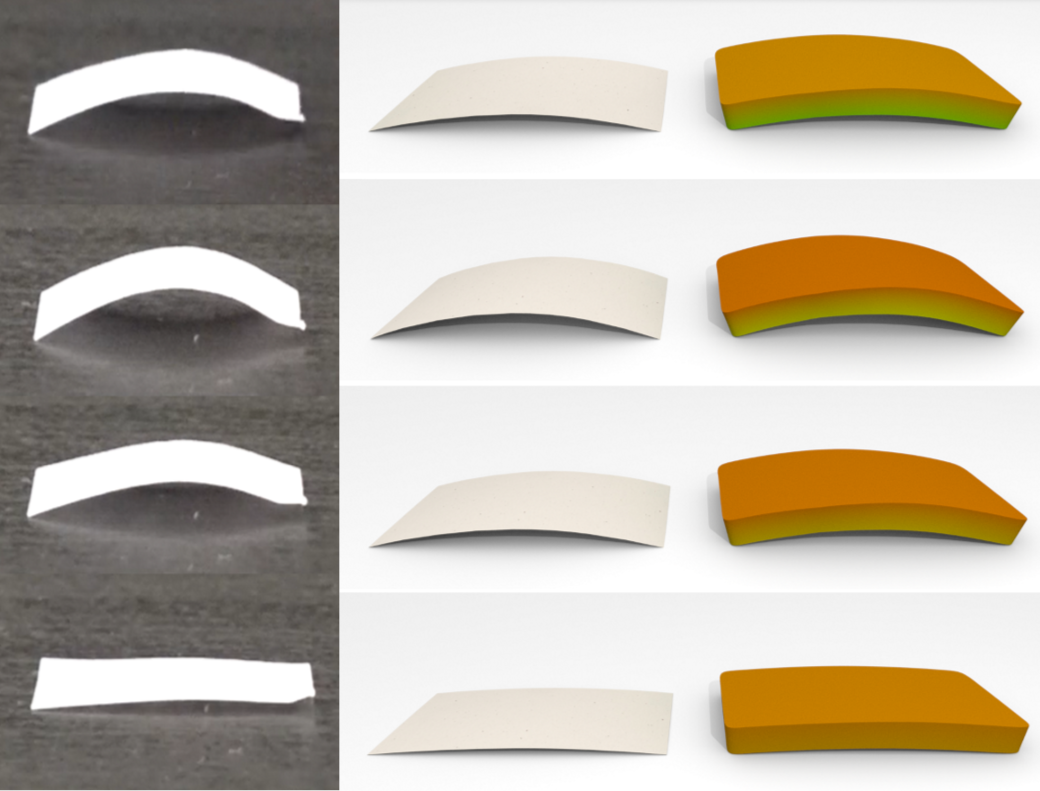
\includegraphics[width=\linewidth]{WaterPainting.png}
  \caption{A comparison between the experiment (left), simulation (middle), and the thickened cross-section (right) as time progresses for a water-painted paper strip. Orange and green indicate high and low moisture content, respectively.}
  \label{WaterPainting}
\end{figure}

We discretize equation~\eqref{eq:diffusion} with bilinear Galerkin finite elements on the triangular prisms $F\times[-h/2,h/2]$; the solution $m$ and source term $s$ in the prism surrounding face $\bff_{ijk}$ are approximated by linear combinations of basis functions 
\begin{align*}
m(u_1,u_2,z) &= \sum_{v\in \{i,j,k\}} \left(m_v^+ \psi_v^+ + m_v^- \psi_v^-\right)\\
s(u_1,u_2,z) &= \sum_{v\in \{i,j,k\}} \left(s_v^+ \psi_v^+ + s_v^- \psi_v^-\right)
\end{align*}
parameterized over the prism $\mathcal{T}\times [-h/2,h/2]$ surrounding the canonical unit triangle. In other words
$$\psi_i^\pm = \frac{(1-u_1-u_2)}{h}\left(\frac{h}{2}\pm z\right); \psi_j^{\pm} = \frac{u_1}{h}\left(\frac{h}{2}\pm z\right); \psi_k^{\pm} = \frac{u_2}{h}\left(\frac{h}{2}\pm z\right).$$
%wim: changed phi to psi since phi is used for embedding
% Formulas for the Galerkin mass and stiffness matrices $M_G$ and $K_G$ are listed in Appendix~\ref{XXX}\todo{Copy in formulas}; 

From the above equations, the moisture is updated each time step using implicit time integration,
\begin{equation}
(M_G+ \Delta t DK_G)\bmm^{i+1} = M_G(\bmm^i + \Delta t \bs^i) \label{eq:discdiffusion}
\end{equation}
where $\bs^i$ is the discretized source term. This source term $\bs_i^{\pm}$ prescribes at each vertex the rate of diffusion of moisture in or out of the shell at both the top and bottom layer of the shell; the details of this term depend on the problem being modeled.

When the mechanism for swelling/shrinking is heat rather than moisture, the above diffusion formulation remains unchanged, with $m$ reinterpreted as temperature rather than moisture.

\section{Numerical Issues}
Integrating the physics~\eqref{eq:implicit} requires some care, as the scale-separation between the stretching and bending forces, along with the very high stiffnesses involved, pose numerical challenges. (The diffusion equation in Equation~\eqref{eq:discdiffusion} poses no numerical difficulties.)
\paragraph{Newton's Method} 
We recommend the usual technique of using the explicit Euler step $\tilde\bv = \bv^{i} + \Delta t\dot\bv^i$ as the initial guess in Newton's method each iteration; writing $\bv^{i+1} = \tilde \bv + \Delta t\delta \bv$, we have from Equation~\ref{eq:implicit}
$$\Lambda\delta \bv - \Delta t \bF\left(\tilde \bv + \Delta t\delta \bv, \bv^{i}\right) = 0 = \sigma(\delta \bv),$$
which is well-scaled for using Newton's method to solve $\sigma(\delta \bv)=0$. The stiffness and nonlinearity of the elastic forces prohibit very large time steps, though a line search allows time integration using $\Delta t\approx 10^{-4}$ seconds.

The Newton gradient $\nabla \sigma = \Lambda + \Delta t^2 \nabla \bF$ is symmetric and almost always positive-definite, and thus amenable to sparse Cholesky decomposition for small-to-medium sized meshes. We use the CHOLMOD solver of the SuiteSparse library~\cite{Chen08} for solving the Newton linear system. In the (rare) cases where $\nabla \sigma$ is detected by the solver to be indefinite, we regularize by using $\nabla \sigma = (1+\alpha)\Lambda + \Delta t^2 \nabla F$ for progressively larger multiples of $\alpha$, until the Cholesky decomposition succeeds. For larger meshes, where the Cholesky factors do not fit in main memory, we solve the equations using Alglib's implementation of LBFGS~\cite{Alglib}. Iterative methods (conjugate gradients) could also be used.
\paragraph{Inexact Hessian} The Hessian of the bending energy is expensive to compute, and almost always dominated by the Hessian of the (much stiffer) stretching term; we observed improved performance replacing the exact bending Hessian with a partial approximation. In particular, we can rewrite the bending energy on face $\bff_{ijk}$ as
\begin{align*}
E_{\mathrm{bending}}(\bv) &= \frac{h^3\sqrt{\det \bar\ba_{ijk}}}{24}\left(r_1(\bv)^2 + r_2(\bv)^2\right)\\
r_1(\bv) &= \sqrt{\alpha/2} \tr\left(\bar\ba_{ijk}^{-1}(\bb - \bar\bb_{ijk})\right)\\
r_2(\bv) &= \sqrt{\beta \tr\left(\left[\bar\ba_{ijk}^{-1}(\bb - \bar\bb_{ijk})\right]^2\right)}
\end{align*}
(note that the trace of the square of any real matrix is guaranteed to be nonnegative). This allows approximation of the Hessian by the Gauss-Newton-esque
$$HE_{\mathrm{bending}} \approx \frac{h^3\sqrt{\det \bar\ba_{ijk}}}{12}\left(\nabla r_1 \nabla r_1^T + \nabla r_2 \nabla r_2^T\right).$$
\paragraph{Inverted Triangles} We observed a somewhat subtle failure case when running simulations containing neighboring triangles with very different prescribed metrics $\bar\ba$: if the two triangles are exactly coplanar, and one triangle collapses completely and inverts, then the mid-edge normal on the common edge is undefined (as its direction is now the mean of two anti-parallel vectors). This failure case can be prevented by either maintaining a minimum vertex/edge/face distance using continuous-time collision detection, by adaptively remeshing triangles undergoing excessive deformation~\cite{Narain2012}, or by adjusting the initial mesh. The usual advice of using an intrinsic Delaunay triangulation, and avoiding adjacent triangles of very disparate size, applies.
\paragraph{Symmetry-Breaking} By symmetry, any rest flat ($\bar\bb=0$) shell has an extrinsically flat equilibrium configuration, regardless of $\bar\ba$. In most cases this equilibrium state is unstable and is not observed in the real world, due to small imperfections in the shell material breaking the symmetry of the initial and/or rest state. We apply a small random perturbation to the rest and initial configurations of all of our initially-flat examples with $\bar\bb=0$, to force symmetry-breaking.

\section{Hinge-Based Shape Operator} \label{sec:gingold}
Gingold et al.~\shortcite{Gingold2004} use a hinge-based shape operator instead, motivated from the observation that on the edges, the shape operator has rank one, and that averaging this per-edge shape operator over an area should yield an approximation to the smooth shape operator. The formulas as originally presented rely fundamentally on the existence of an embedded, Euclidean undeformed mesh, and so it is not obvious how to extend the formulation to the non-Euclidean setting where arbitrary $\bar\ba$ and $\bar\bb$ are prescribed. One possible extension of Gingold et al.'s formula is
$$S_{\mathrm{gingold}}(\bm{\theta}) = \sum_{i=1}^3 \frac{\sqrt{\bw_i^T \bar\ba\bw_i} \tan\left(\theta_i/2\right)}{\|\bw_i\|^2\sqrt{\det\bar\ba}} \bw_i \bw_i^T$$
which takes into account length and area distortions of the triangle's rest pose due to the metric $\bar\ba$. Here $i$ sums over the three edges of the canonical barycentric triangle $\mathcal{T}$; $\bw_i$ is the vector normal to edge $i$ and with magnitude equal to that of edge $i$, and $\theta_i$ is the hinge angle associated to edge $i$. Given rest hinge angles $\bar\theta_i$, the difference $S_{\mathrm{gingold}}(\bm{\theta}) - S_{\mathrm{gingold}}(\bar{\bm{\theta}})$ can be substituted in for $\bar\ba^{-1}(\bb-\bar\bb)$ in the Koiter energy. We compare this formulation, to the one above based on the mid-edge shape operator, in section~\ref{comparisons} below.

\paragraph{Solving for Hinge Angles} Given a desired $\bar\bb$, rest angles $\bar\theta_i$ can be recovered by evaluating the shape operator in test directions $\bw_i$: we desire
$$\frac{\bw_i^T \bar\bb \bw_i}{\bw_i \bar\ba \bw_i} = \bw_i^T S_{\mathrm{gingold}}(\bar{\bm{\theta}}) \bw_i, \quad i\in\{1,2,3\},$$
a system of three linear equations in $\tan(\bar\theta_i/2)$. Note that two neighboring faces might disagree on the value of the rest hinge angle of their common edge; to support non-Euclidean rest geometry, both values must be stored and used when computing the energy density of their respective triangles.

\section{Results}
We evaluate the simulation on a variety of examples, both didactic and complex.

\subsection{Analytic Benchmarks}
We first test the method on examples where the equilibrium state can be computed exactly. When an embedding $\br$ exists for which $\ba = \bar \ba$ and $\bb = \bar\bb$, that embedding is clearly a global minimizer of the elastic energy, regardless of material parameters. We ran all of the following experiments using the default values in Table~\ref{tab:params}. We ran the simulation for enough time to reach steady state.

\begin{figure}[h]
  \centering
  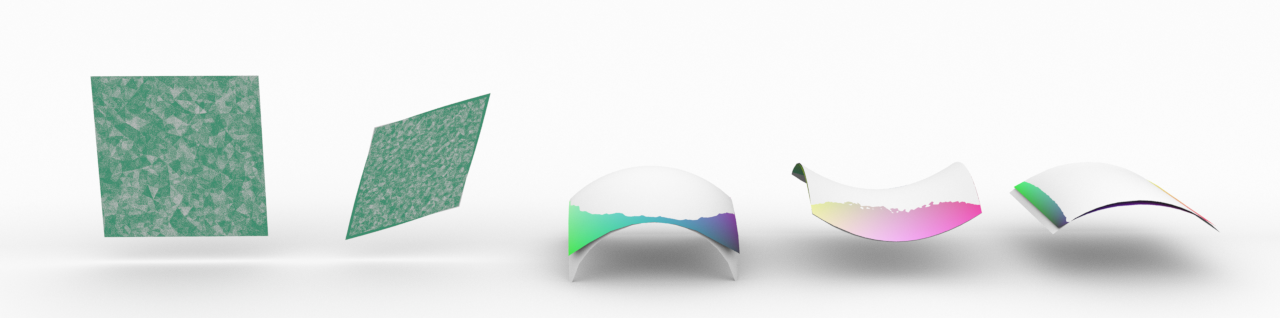
\includegraphics[width=0.5\textwidth]{didactic.png}
  \caption{The exact solutions (white) and simulated surfaces (colored) from the didactic examples. From left to right are the enlarged square, rhombus, spherical cap, hyperboloid, and cylindrical patch experiments.}
  \label{fig:didactic}
\end{figure}
\paragraph{Swelling of Square} We take $\Omega$ to be a unit square, with $\br=\Id$, and assign static fields for both $\bar\ba$ and $\bar\bb$ to the entire shell. Table~\ref{tab:analytic} summarizes the values of $\bar\ba$ and $\bar\bb$ we tried, and the expected shape and curvatures of the exact solution. In cases where $\bar\bb=0$ and $\bar\ba$ is homogenous over the surface, our method must (and does) reproduce the exact solution. Examples with rest curvature are affected by discretization error; we ran the simulation using three mesh resolutions (XXX/YYY/ZZZ vertices) and for each, plot the distance of each point from the corresponding point on the exact solution in Figure~\ref{fig:didactic}.
\begin{table*}
\begin{tabular}{cclccccc}
$\bar\ba$ & $\bar\bb$ & Expected Shape & Mean Curv.  & Gauss Curv. & Error (one-sided Hausdorff) \\
$4\Id$ & $0$ & Enlarged Square & $0$ & $0$ & XXX \\
{\scriptsize $\frac{1}{1-x^2-y^2}\begin{pmatrix}1-y^2 & xy\\ xy & 1-x^2\end{pmatrix}$} & {\scriptsize $\frac{1}{1-x^2-y^2}\begin{pmatrix}1-y^2 & xy\\ xy & 1-x^2\end{pmatrix}$ } & Spherical Cap & $1$ & $1$  & XXX \\
{\scriptsize $\begin{pmatrix}1+x^2 & -xy \\ -xy & 1+y^2\end{pmatrix}$ } & {\scriptsize $\frac{1}{\sqrt{1+x^2+y^2}}\begin{pmatrix}-1 & 0\\0 & 1\end{pmatrix}$ } & Hyperboloid Cap & varies & $<-1$ & XXX/XXX/XXX \\
$\begin{pmatrix}2 & 1\\1 & 2\end{pmatrix}$ & 0 & Rhombus & $0$ & $0$ & XXX/XXX/XXX \\
$\Id$ & $\begin{pmatrix} 1 & 0\\0 & 0\end{pmatrix}$  & Cylindrical Patch & $1$ & $0$ & XXX/XXX/XXX
\end{tabular}
\caption{Didactic experiments on a unit square. Different $\bar\ba$ and $\bar\bb$ are prescribed over the square, and in each case we compare the simulated steady state to the expected analytic solution.}
\label{tab:analytic}
\end{table*}

\paragraph{Isotropic Growth} The Riemann mapping theorem guarantees that every surface $M$ with disk topology can be parameterized by the unit disk, with metric conformally equivalent to the Euclidean metric. This insight was exploited by Kim et al~\shortcite{Kim2012} to grow an approximate sphere from a square. 

When $M$ is not flat, we do not expect the shell to grow \emph{exactly} into the shape $M$, since embedding the shell as the shape $M$ minimizes stretching energy while ignoring bending energy. Nevertheless, we expect the steady state geometry to closely resemble $M$, especially when $M$ is convex and the shell thickness $h$ is small. Figure~\ref{ContractingSphere} shows the result of swelling the unit disk into a sphere: we stereographically project the sphere of radius $1/4$ units to the plane, and take the region bounded by the unit disk. Stereographic projection is conformal, so we set $\bar\ba$ on the unit disk per the conformal factor, and simulate the damped dynamics of the disk returning to its equilibrium state. Notice that the disk transitions through highly deformed intermediate states before ``popping'' back into a spherical shape. The rest state is not perfectly spherical at the boundary: the shell flares outward, as expected since the perfectly spherical configuration minimizes stretching energy while neglecting bending. A theoretical argument for this behavior at the boundary is given in \cite{Efrati2009_2}.

\paragraph{Comparison to Finite Elements}
We compare our method to finite elements to validate both the discretized elastic energy, and the equilibrium configuration, of a slab undergoing differential non-Euclidean growth. More specifically, for different growth magnitudes $G$ we prescribe the rest metric
$$\bar\bg = \left [\frac{(1 + G)z}{h} + \left(1 - \frac{z}{h}\right)\right]^2$$
throughout the volume of a 20 by 10 mm slab of thickness $h=0.1$ mm, and evaluate its elastic energy using three methods: (i) tetrahedral finite elements using a St. Venant-Kirchhoff material model, where each tetrahedron is assigned a piecewise constant rest metric by evaluating $\bar\bg$ at its centroid; (ii) our method, as described in section~\ref{sec:discretization}; (iii) our method, using Gingold et al.'s hinge-based shape operator, as discussed in section~\ref{sec:gingold}. All finite element energies and simulations were computed using the Vega library~\cite{Vega}. We also compute two ground truth energy values: the true elastic energy of a St. Venant-Kirchhoff material integrated over the shell volume, and the energy of the midsurface-based thin limit approximation in equation~\ref{eq:koiter}. 
Figure~\ref{fig:Convergence} shows convergence plots of the elastic energy of the finite element and shell methods as a function of mesh resolution. For a fixed value $G=0.03$, we compute the energy of a non-equilibrium embedding of the slab $\br(x,y) = XXX$. Both shell-based methods converge quadratically (albeit to different limit energies) with the mid-edge operator formulation more accurate in the limit. Figure~\ref{fig:validation} plots the error of both shell methods relative to the FEM solution, for different levels of refinement; on a coarse mesh our method slightly underestimates the curvature of the FEM solution; the formulation using Gingold et al.'s operator overestimates it.

Table~\ref{tab:energy} compares the limit energy values of the discrete methods to the ground truths, for different values of $G$ (the meshes used for this experiment contain 22881 tetrahedra/ 5538 triangles).  Our method shows good agreement with the Koiter energy. Notice that for high values of $G$, even the exact Koiter energy does not agree with the true volumetric elastic energy; this is because as $G$ grows large, the modeling assumption that strain is small relative to the thickness of the shell no longer holds. 
\begin{table*}
\begin{tabular}{l|ccccccc}
method & $G=0.005$ & $0.03$ & $0.05$ & $0.08$ & $0.1$ & $0.3$ & $0.5$  \\
\hline
True Volumetric Energy & $1.6x10^{-6}$ & $5.64x10^{-5}$ & $1.55x10^{-4}$ & $3.87x10^{-4}$ & $5.974x10^{-4}$ & $4.77x10^{-3}$ & $1.2x10^{-2}$ \\
Thin Limit Approximation & XXX &\\
\hline
Our Energy & $1.6x10^{-6}$ & $5.77x10^{-5}$ & $1.6x10^{-4}$ & $4.1x10^{-4}$ & $6.4x10^{-4}$ & $5.67x10^{-3}$ & $1.54x10^{-2}$ \\
Hinge-based Formulation & $2.2x10^{-6}$ & $8.01x10^{-5}$ & $2.29x10^{-4}$ & $6.11x10^{-4}$ & $9.83x10^{-4}$ & $1.23x10^{-2}$ & $5.01x10^{-2}$ \\
Volumetric Finite Elements & XXX
\end{tabular}
\caption{Comparison of the elastic energy of a thin slab, simulated using tetrahedral finite elements, our method using the mid-edge shape operator, and using Gingold's hinge-based shape operator. Higher $G$ induces more differential growth.}
\label{tab:energy}
\end{table*}

\begin{figure}[h]
  \centering
  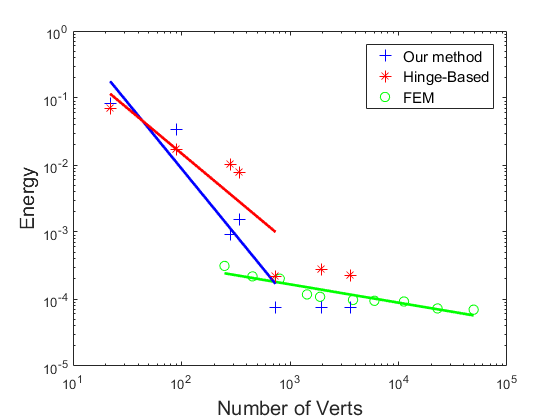
\includegraphics[width=\linewidth]{Convergence.png}
  \caption{ Comparision of energy convergence rate as a function of resolution of our method, hinge-based method, and FEM}
  \label{fig:Convergence}
\end{figure}

\subsection{Comparisons to Experiments}
We validate our simulated results against several real-world experiments.
\paragraph{Curling of Paper}
Ordinary paper, when moistened on one side (by painting water on the top side, or placing the bottom side on a damp sponge), undergoes complex dynamic behavior. Water diffuses into the wet side, and that side swells, causing the paper to globally curl up out of plane due to this differential material growth. Over time, water penetrates the entire thickness of the paper and the water concentration becomes uniform; the paper flattens again. This process plays out over a time scale of about ten seconds. We compare experiment and simulation of this behavior, for a rectangular paper strip of dimensions. We use a brush to moisten a piece of real paper, and compare the video of the curling and uncurling of the paper to a simulation of the same phenomenon. Figure~\ref{WaterPainting} shows the experiment, the simulation, and a stylized, thickened cross-section of the paper showing the difference in moisture concentration through the paper thickness over time.

\paragraph{Radial Swelling of Disk}
Sharon and Efrati~\shortcite{Sharon2010}, in their pioneering work on the geometry of non-Euclidean plates, induced non-uniform growth in a punctured disk of NIPA polymer by varying the cross-linking ratio as a function of the radius away from the disk's center. Our simulations are able to reproduce the geometries they observed experimentally. Figure~\ref{SwellingDisc} compares experiment and simulations.

\begin{figure}[h]
  \centering
  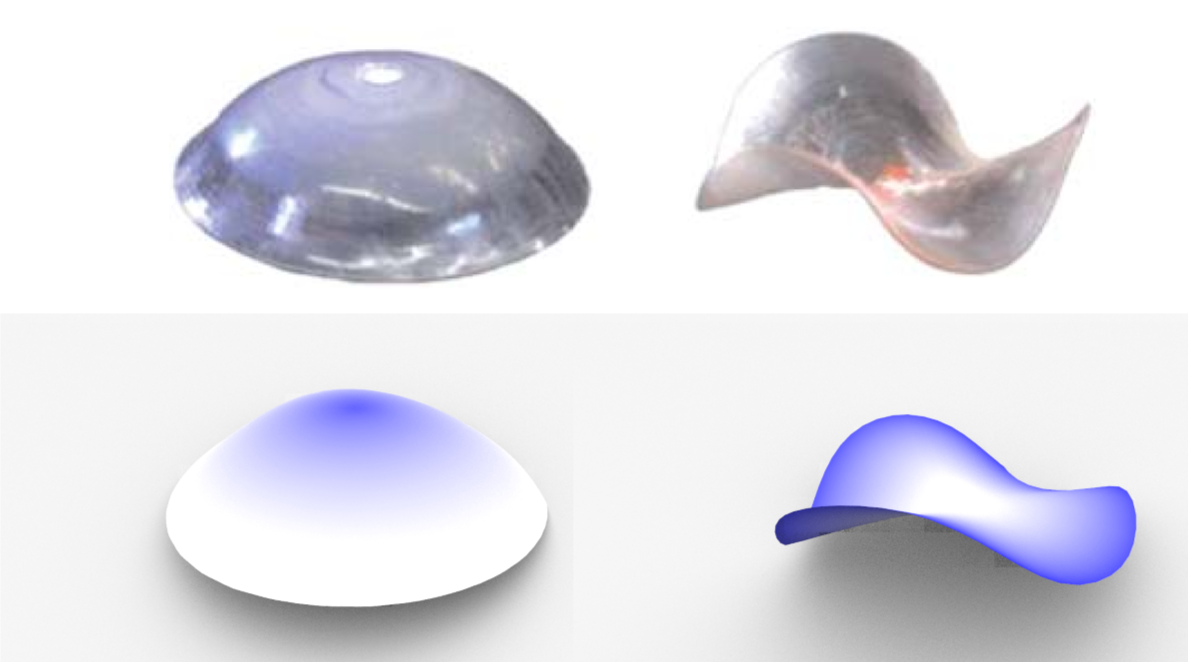
\includegraphics[width=\linewidth]{SwellingDisc.png}
  \caption{We compare the experimental result by Sharon and Efrati~\shortcite{Sharon2010} using polymer disks (top) with our simulation (bottom) for two different prescribed radially-varying rest metrics. Blue regions correspond to higher growth rates. }
  \label{SwellingDisc}
\end{figure}

\subsection{Effects of Parameters}
One advantage of our formulation of swelling thin shells is that it supports physical material parameters. In this section, we show results highlighting the importance of these parameters and their effects on the behavior of swelling and shrinking thin objects.

\paragraph{Thickness}
Since it controls the relative importance of stretching and bending, the thickness of a shell is its most important physical parameter. Changing the thickness will often dramatically change how a shell deforms. For example, when a moist paper annulus dries, it rolls up. Depending on its thickness, the annulus transitions through several intermediate shapes before rolling up completely: the outer boundary of the annulus lifts to form an $n$-sided polygon, with $n$ decreasing over time as one metastable configuration cascades into the next. Figure~\ref{Annuli} shows the range of behavior for an annulus of inner radius $1$ cm and outer radius $2$ cm, and several paper thicknesses ($0.05$, $0.1$, $0.2$ and $0.5$ mm).

\paragraph{Machine Direction}
As mentioned above, when paper is manufactured, paper fibers tend to be arranged in a preferential direction, leading to anisotropic growth when the paper is moistened. In figure~\ref{Annuli} (right) we repeat the annulus experiment with paper whose fibers are aligned to the $x$ direction (left to right in the figure). Notice the dramatic change in the annulus dynamics, compared to Figure~\ref{Annuli} (left).

\begin{figure}[!h]
%\begin{minipage}[t]{0.45\linewidth}
%    \centering
 %   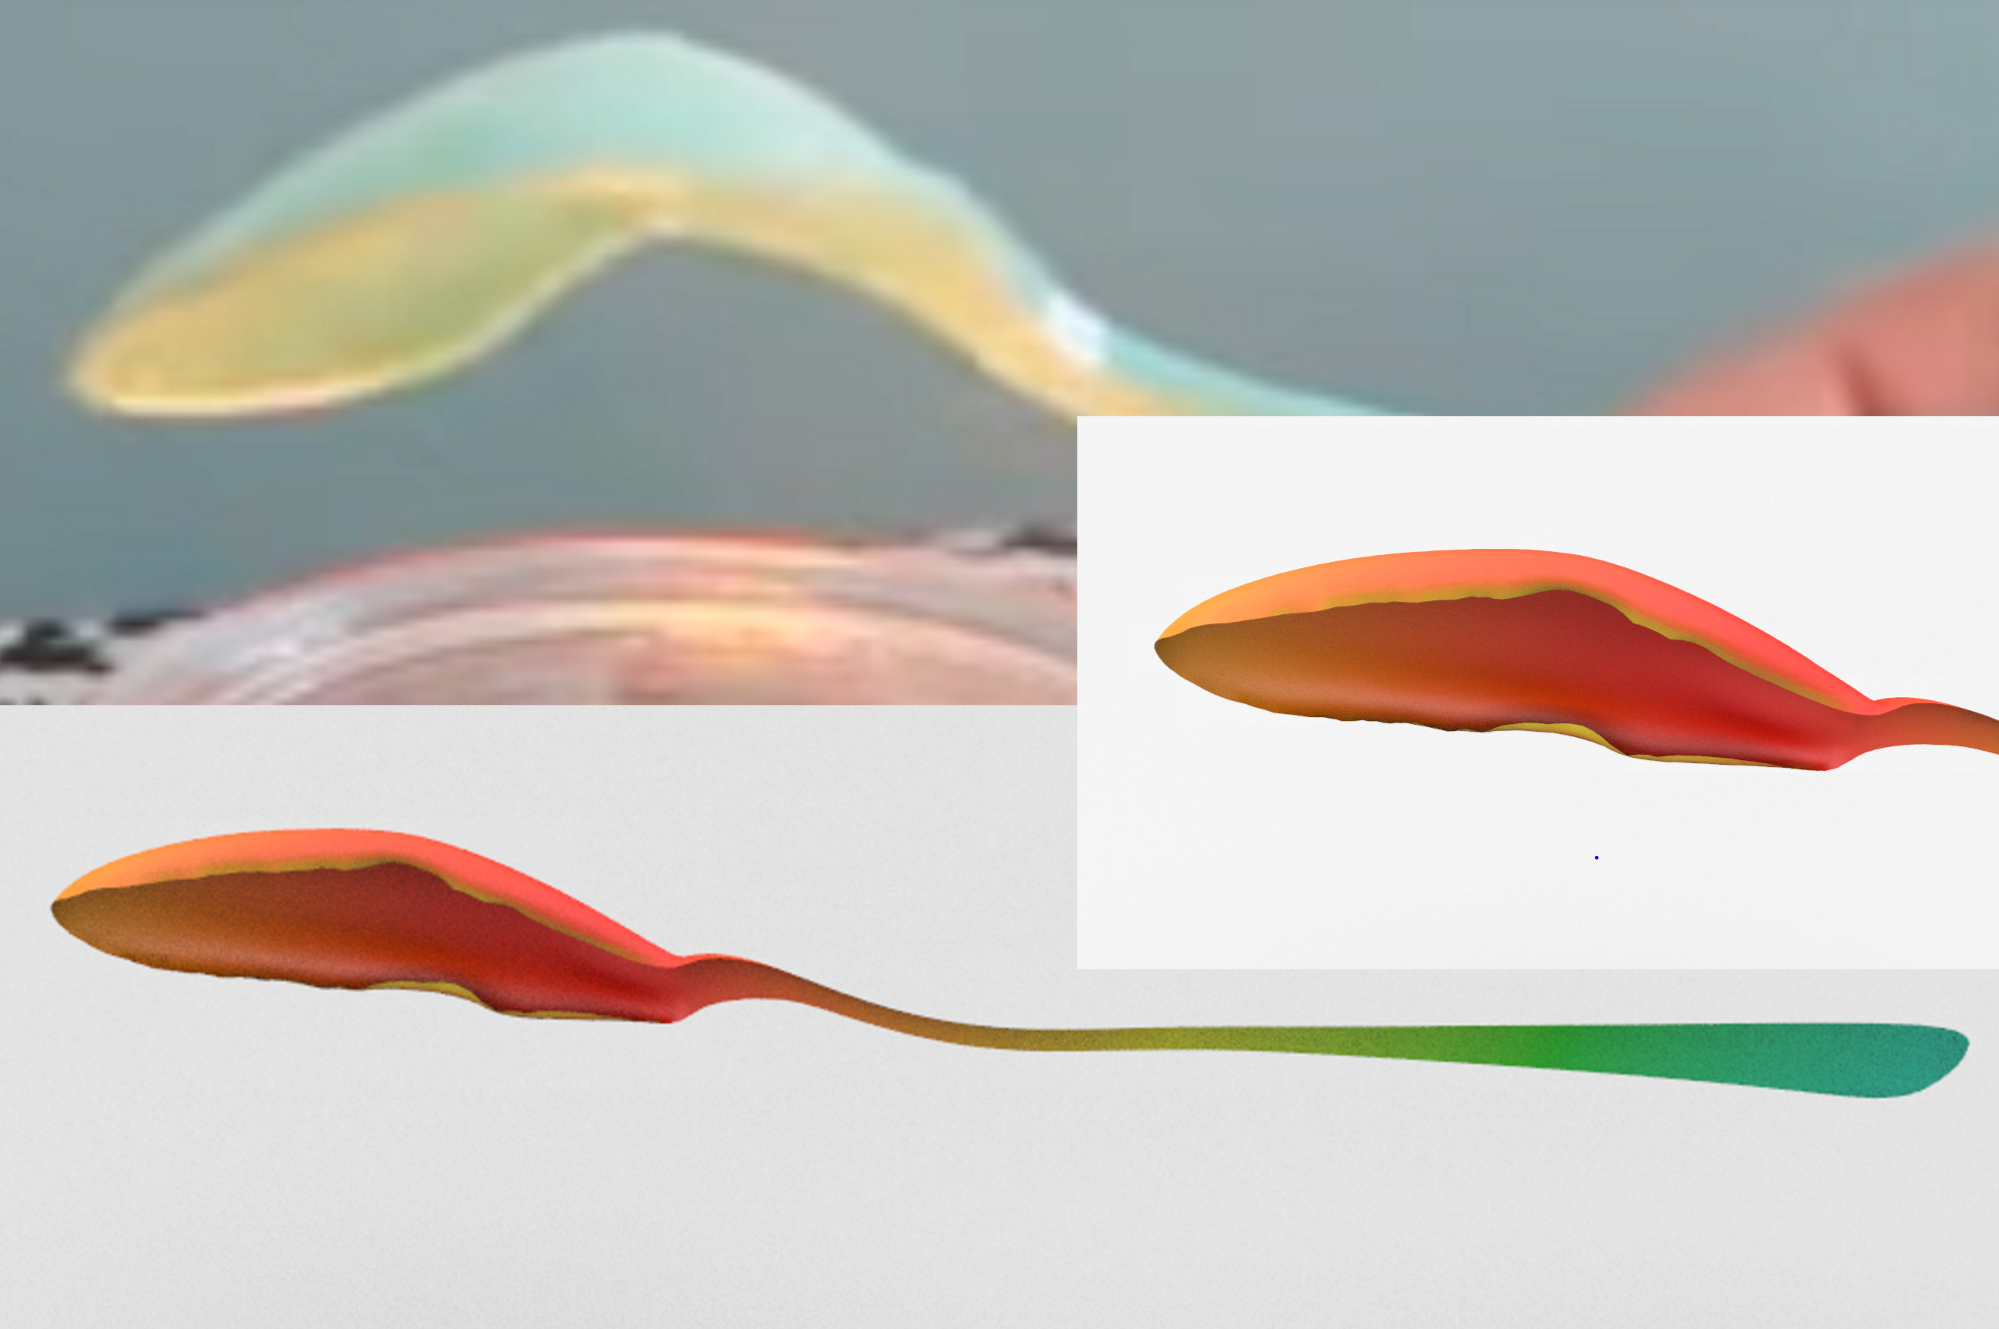
\includegraphics[width=1\textwidth]{Spoon.png}
 %   \caption{When a spoon is heated, its head buckles and crumped. This figure shows a real world experiment (top), our simulated spoon (bottom) where hotter parts are redder, and an inset of focusing on the distorted front of the spoon.}
%    \label{Spoon}
%\end{minipage}
%\hspace{0.1cm}
\begin{minipage}[t]{0.45\linewidth} 
    \centering
    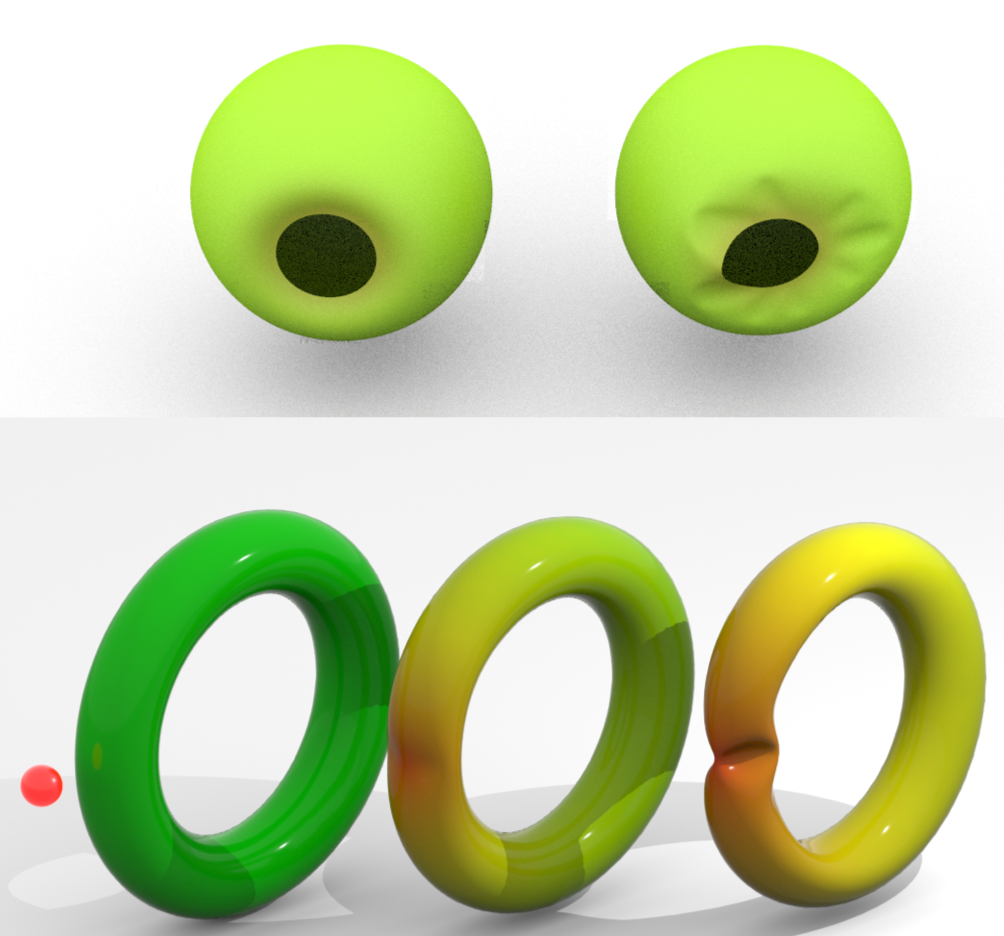
\includegraphics[width=1\textwidth]{TorusandSphere.png}
    \caption{Deformed punctured plastic spheres with different temperature distribution with hotter region indicated as red are shown on the top panel. Plastic torus deformation due to heat source (red sphere) through time is shown in the bottom. }
    \label{fig:TorusandSphere}
\end{minipage}        
\end{figure}

\begin{figure*}[h]
  \centering
  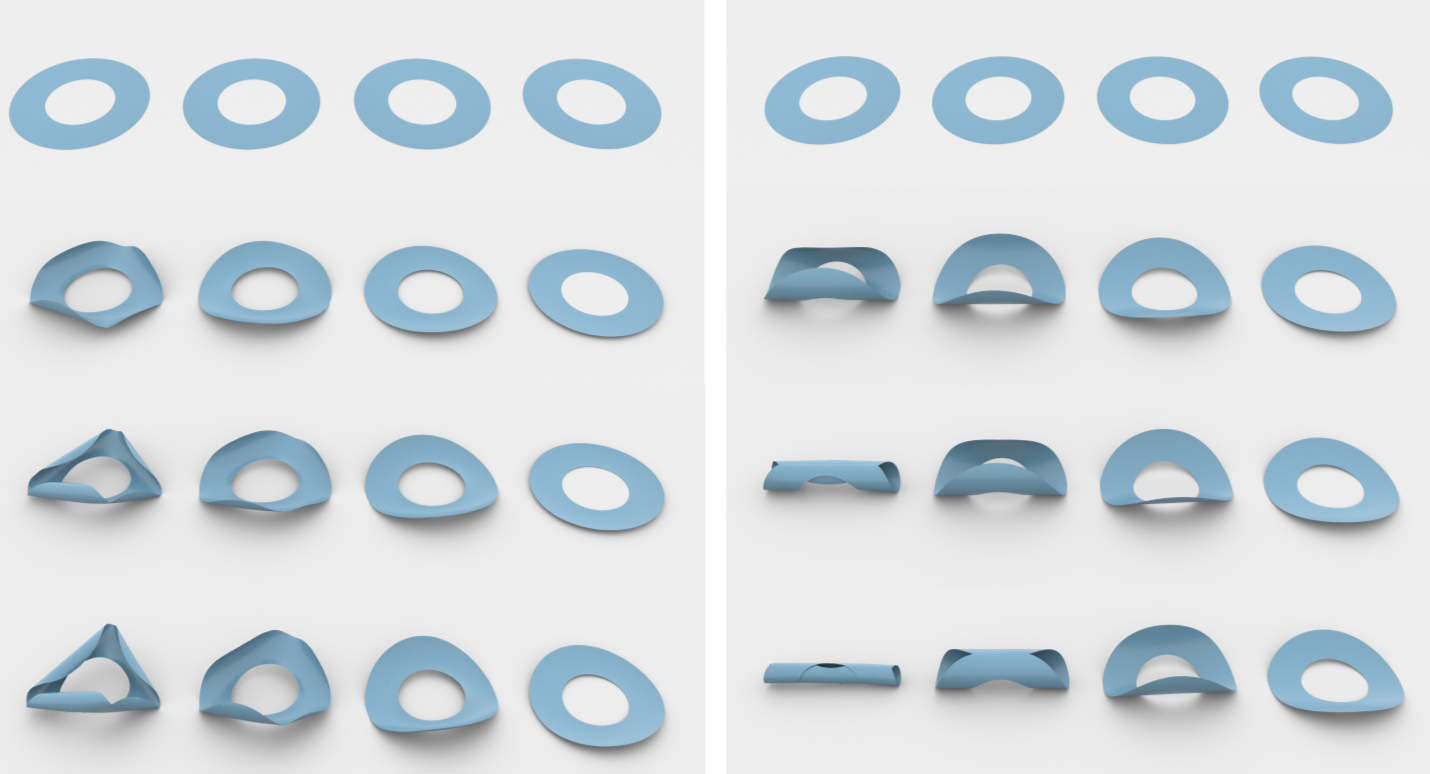
\includegraphics[width=\textwidth]{Annuli.png}
  \caption{The left figure shows the curling behavior of moist paper annuli as they dry, with time increasing from top to bottom. Varying the thickness (from left to right, the thicknesses of the annuli are 0.05 mm, 0.1 mm, 0.2 mm, and 0.5 mm) demonstrates that the amount and type of curling is strongly dependent on the thickness of the material. The right figure shows the same annuli endowed with a principal machine direction along the $x$ axis (directed from left-to-right in the figure): the dynamics are markedly different from the case of no machine direction. }
  \label{Annuli}
\end{figure*}

\subsection{Qualitative Experiments}
We end with several experiments that demonstrate the flexibility of the method to simulate complex geometries undergoing nonlinear deformations due to differential swelling along with the timing required to generate a frame in table ~\ref{tab:timing}.

\begin{table}[htb]
\begin{tabular}{lc|cc|cc}
Example & Fig & verts & tris & time step (s) & time/step (s) \\
\hline
Bunny & \ref{fig:BunnyandArmadillo} & 51k & 102k & $10^{-5}$ & 5.25  \\
Armadillo & \ref{fig:BunnyandArmadillo} & 42k & 86k &  $10^{-5}$ & 33.88 \\
Pasta & \ref{fig:pasta} & 9k & 19k & $10^{-4}$ &  23.6 \\
Globe & \ref{SwellingDisc} & 5k & 10k & & \\
Annuli  & \ref{Annuli} & 1.5k & 3k & $10^{-4}$ & 8 
\end{tabular}
\caption{Timing numbers for the simulations shown in the paper. All simulations were run on an XXX desktop using one thread.}
\label{tab:timing}
\end{table}

%\paragraph{The Spoon}
%Common plastic spoons are made of polypropylene, a thermoplastic which shrinks when heated. Applying heat to the curved portion of a spoon thus induces a dramatic change in shape; figure~\ref{Spoon} compares a simulation of this process to video of a real-world experiment~\cite{youtube}.

\paragraph{Shape-changing Food} Differential growth has been used to design gelatin films that fold into novel shapes, by exploiting the ability to fabricate the film into a bilayer of differing density and porosity~\cite{Wang2017}. Wang et al. validated their designs using a volumetric simulation in ABAQUS; in figure~\ref{fig:pasta} we compare their simulated and experimental results to our thin shell simulations, demonstrating that a reduced shell model can accurately predict the behavior of the bilayer without need of a volumetric simulation.

\paragraph{Melting Plastic} We simulate the behavior of several thin-shell plastic objects (sphere, torus bunny, and armadillo) shrinking when exposed to heat. Notice the complex buckling patterns visible in these examples, due to metric incompatibility introduced into the object geometry during heating. See figure~\ref{fig:BunnyandArmadillo} and figure~\ref{fig:TorusandSphere}.

\clearpage
\bibliographystyle{ACM-Reference-Format}
\bibliography{MoistSim}
\end{document}

